\documentclass[10.5pt,a4paper]{article}
\usepackage[utf8]{inputenc}
\usepackage[T1]{fontenc}
\usepackage{lmodern,microtype}
\usepackage[margin=19mm]{geometry}
\usepackage{amsmath,amssymb,booktabs,graphicx,xcolor,enumitem,float,caption,subcaption}
\usepackage[colorlinks=true,allcolors=black]{hyperref}
\setlist{itemsep=2pt,topsep=3pt,leftmargin=*}
\captionsetup{font=small,labelfont=bf}
\newcommand{\cm}{\,cm}

\title{\vspace{-12mm}\textbf{Single-LED 3D Visible Light Positioning with a Single Reorientable Photodiode}\\[2pt]
\large Experimental results - Summary}
\author{Kevin Acuna-Condori}
\date{October 20, 2026}

\begin{document}
\maketitle
\vspace{-6mm}

\section*{Highlights}
\vspace{-2mm}\noindent\rule{\linewidth}{0.4pt}
\begin{itemize}[leftmargin=4mm]
\item \textbf{3.7\cm\ mean 3D error with a single LED and a single photodiode.} Over 125 positions on
  5 heights (median 3.4\cm, P90 6.1\cm, no failures), with $K=10$ orientations. With $K=5$ the error is
  the same (3.7\cm); with $K=3$ it is 4.9\cm.
\item \textbf{Validated live.} The real-time demo on 131 random, blind positions ($K=5$) gives 4.1\cm\
  (median 3.9\cm).
\item \textbf{Calibration needs only 9 positions.} A $3\times3$ grid over the working area, with a flat
  PD, gives 3.5\cm, the same as the 19\,881-point map. It also yields the LED $XY$ position.
  \emph{Where} the points are matters more than \emph{how many}: 9 points clustered around the LED
  give 17--22\cm.
\item \textbf{The positioning system diagnosed its own testbed.} From the RSS alone, VLP revealed that
  the gantry $Z$ axis travels only $\approx 0.63\times$ the commanded distance. A tape measurement
  later gave $0.6\times$. Correcting it halves the error (7.1 $\rightarrow$ 3.7\cm).
\item \textbf{The 700\,kHz LED is tilted by $\approx 5^\circ$.} Its radiation pattern is centred
  18\cm\ away from its physical position, so the method is a diagnostic tool for the installation too.
\item \textbf{The photodiode angular model is decisive.} The SQ response (Bastiaens 2020) gives
  3.9\cm; the usual $\cos^{m_R}$ and Lambertian $\cos$ models give 8.4\cm\ and 77\cm.
\item \textbf{Two LEDs give position and yaw without any power calibration.} Intersecting the
  directions to two LEDs, the minimum for crossing rays (e.g.\ a corridor), needs no LED gain and no
  Lambertian order. With the best pair (500 + 900\,kHz) the error is 3.3\cm\ with known yaw, and
  3.6\cm\ with the yaw estimated too (1.2$^\circ$ yaw error). This is a path to IMU-free attitude.
\end{itemize}
\noindent\rule{\linewidth}{0.4pt}

\section*{1. Setup in brief}
\begin{itemize}
\item \textbf{Single-LED system.} The system under study uses \textbf{one LED} on the ceiling (3.0\,m,
  facing down, modulated at 500\,kHz). All results refer to this LED unless stated otherwise.
\item \textbf{Receiver.} A Thorlabs PDA100A2 photodiode on a $15^\circ$ adapter, turned by a motorized
  rotation stage to $K$ azimuths.
\item \textbf{Additional LEDs, for comparison only.} The testbed has three more LEDs (300, 700 and
  900\,kHz). Their RSS is recorded in the same measurements by frequency separation. They are used only
  in the comparisons with two or more LEDs (F6) and for the installation diagnosis (F5).
\item \textbf{Ground truth.} An igus XYZ gantry: $1.4\times1.4$\,m, PD height 0.95--1.32\,m.
\item \textbf{RSS measurement.} Lock-in on 100\,ms raw records (1\,Mpts, Keysight MSO-X 4154A).
\item \textbf{Estimator.} The direction comes from the \emph{shape} of the $K$ RSS (NLS, SQ PD
  response). The range is in closed form from the same RSS, with the calibrated LED gain $A$ and
  Lambertian order $m$.
\item \textbf{Datasets.}
  \begin{itemize}
  \item 125 positions $\times$ $K=10$ (1\,250 measurements, regular $5\times5$ grid $\times$ 5
    heights);
  \item a flat-PD RSS map of 19\,881 points (10\,mm grid);
  \item 131 random positions from the live demo;
  \item the link frequency response (5\,kHz--1\,MHz).
  \end{itemize}
\item \textbf{Tooling.} The acquisition tool and the demo run unattended for many hours. Raw-socket
  SCPI over LAN replaced the vendor VISA, whose large transfers froze the oscilloscope: 1\,500
  consecutive 1-Mpt captures ran without error. Interrupted campaigns recover automatically and can be
  resumed.
\end{itemize}

\section*{2. Main results}
\begin{table}[H]\centering\small
\begin{tabular}{lcccc}\toprule
Configuration (500\,kHz LED unless stated) & Positions & Mean & Median & P90\\\midrule
Single LED, $K=10$, regular 3D grid & 125 & \textbf{3.66} & 3.40 & 6.05\\
\quad $K=5$ (all subsets of the 10 angles) & 125 & 3.73 & 3.56 & 5.94\\
\quad $K=3$ & 125 & 4.94 & 4.70 & 8.07\\
Calibrated with only 9 points ($3\times3$), LED $XY$ known & 125 & 3.54 & 3.17 & 6.48\\
Calibrated with only 9 points, LED $XY$ also calibrated & 125 & 3.47 & 3.13 & 6.35\\
Live demo, random positions, $K=5$ & 131 & 4.10 & 3.91 & 6.68\\
Two LEDs (500 + 900\,kHz), directions only (no $A$, $m$) & 50 & \textbf{3.30} & 2.50 & 6.27\\
\quad same, yaw unknown and estimated & 50 & 3.60 & 3.06 & 7.03\\
Four LEDs, directions only & 50 & 2.77 & 2.46 & 5.34\\
\quad same, yaw unknown and estimated & 50 & 2.92 & 2.50 & 5.33\\\midrule
\multicolumn{5}{l}{\emph{What happens if a model element is wrong} (mean error, same 125 positions):}\\
Gantry $Z$ taken as commanded (no 0.6 scale) & \multicolumn{4}{l}{7.1\cm\ (vertical bias from $-12$ to $+9$\cm)}\\
PD response $\cos^{1.9}\psi$ / $\cos\psi$ instead of SQ & \multicolumn{4}{l}{8.4\cm\ / 77\cm}\\
Calibration points clustered around the LED ($3\times3$, 0.2\,m) & \multicolumn{4}{l}{17.3\cm}\\\bottomrule
\end{tabular}
\caption{3D positioning error in cm. The multi-LED rows use the 50 positions of the first campaign (on
those positions the single-LED method gives 2.98\cm), with the positions of the other LEDs obtained from
their ray intersections at the other height.}
\end{table}

\begin{figure}[H]\centering
\begin{subfigure}{0.49\linewidth}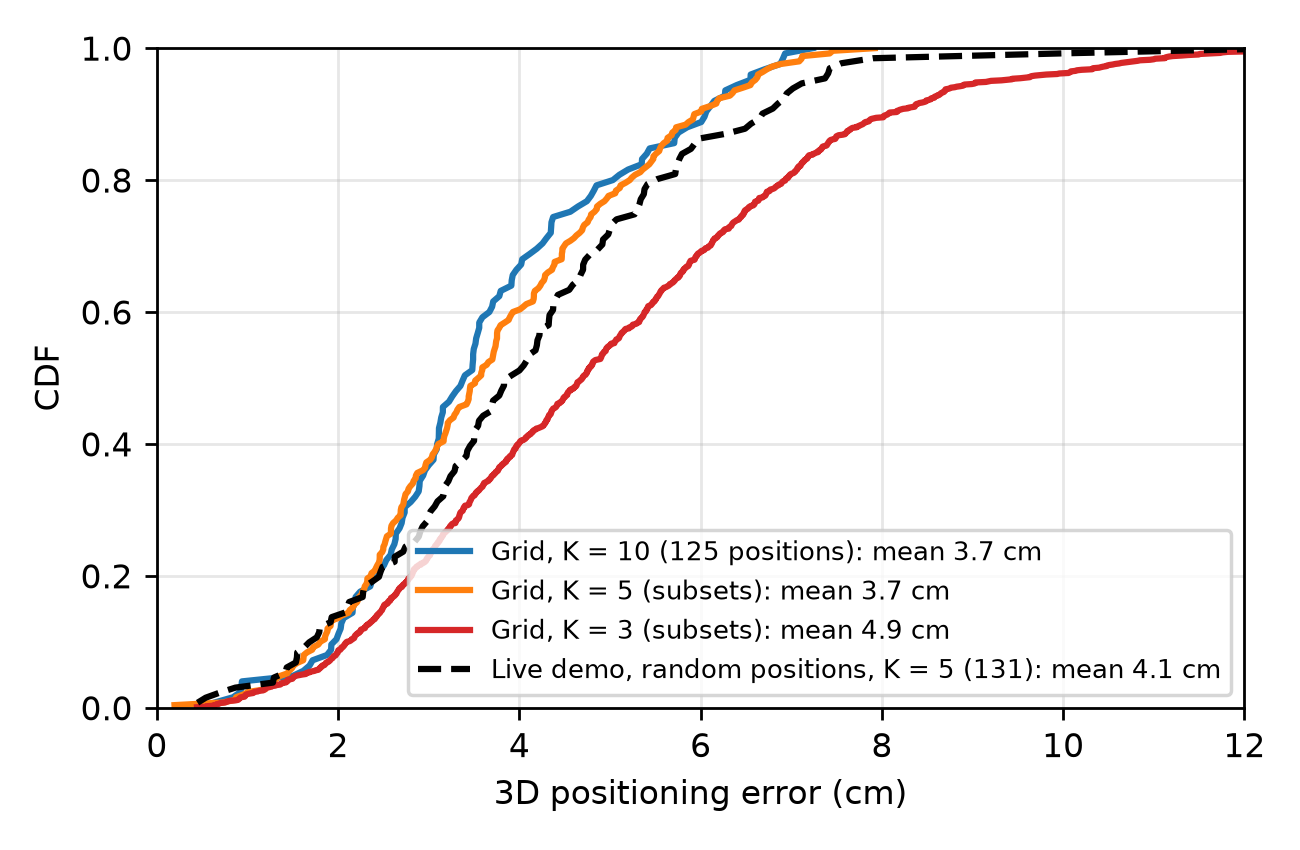
\includegraphics[width=\linewidth]{fig_accuracy.png}
\caption{Error CDF: regular grid ($K$ = 10, 5, 3) and live demo.}\end{subfigure}\hfill
\begin{subfigure}{0.49\linewidth}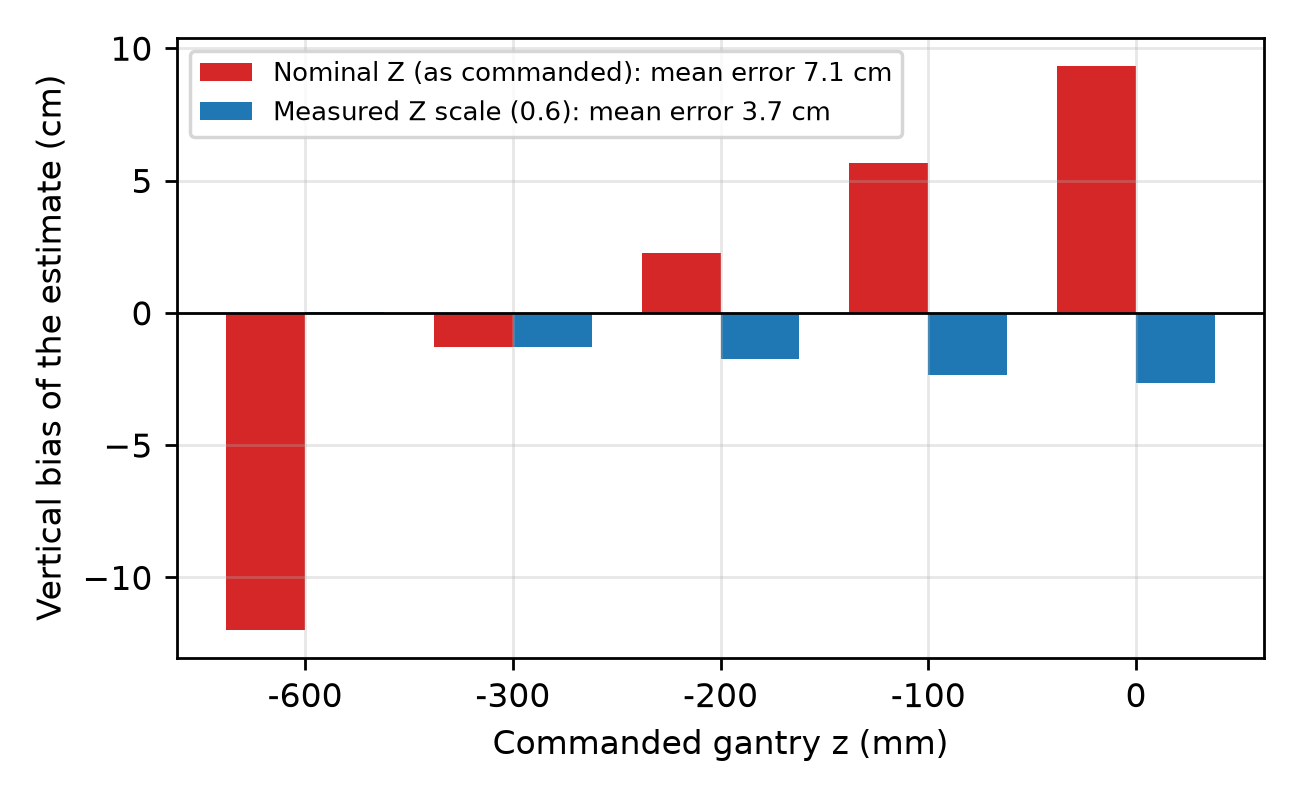
\includegraphics[width=\linewidth]{fig_zaxis.png}
\caption{Vertical bias per gantry height: nominal $Z$ vs. measured scale.}\end{subfigure}
\caption{Accuracy and the gantry $Z$-axis diagnosis.}
\end{figure}

\begin{figure}[H]\centering
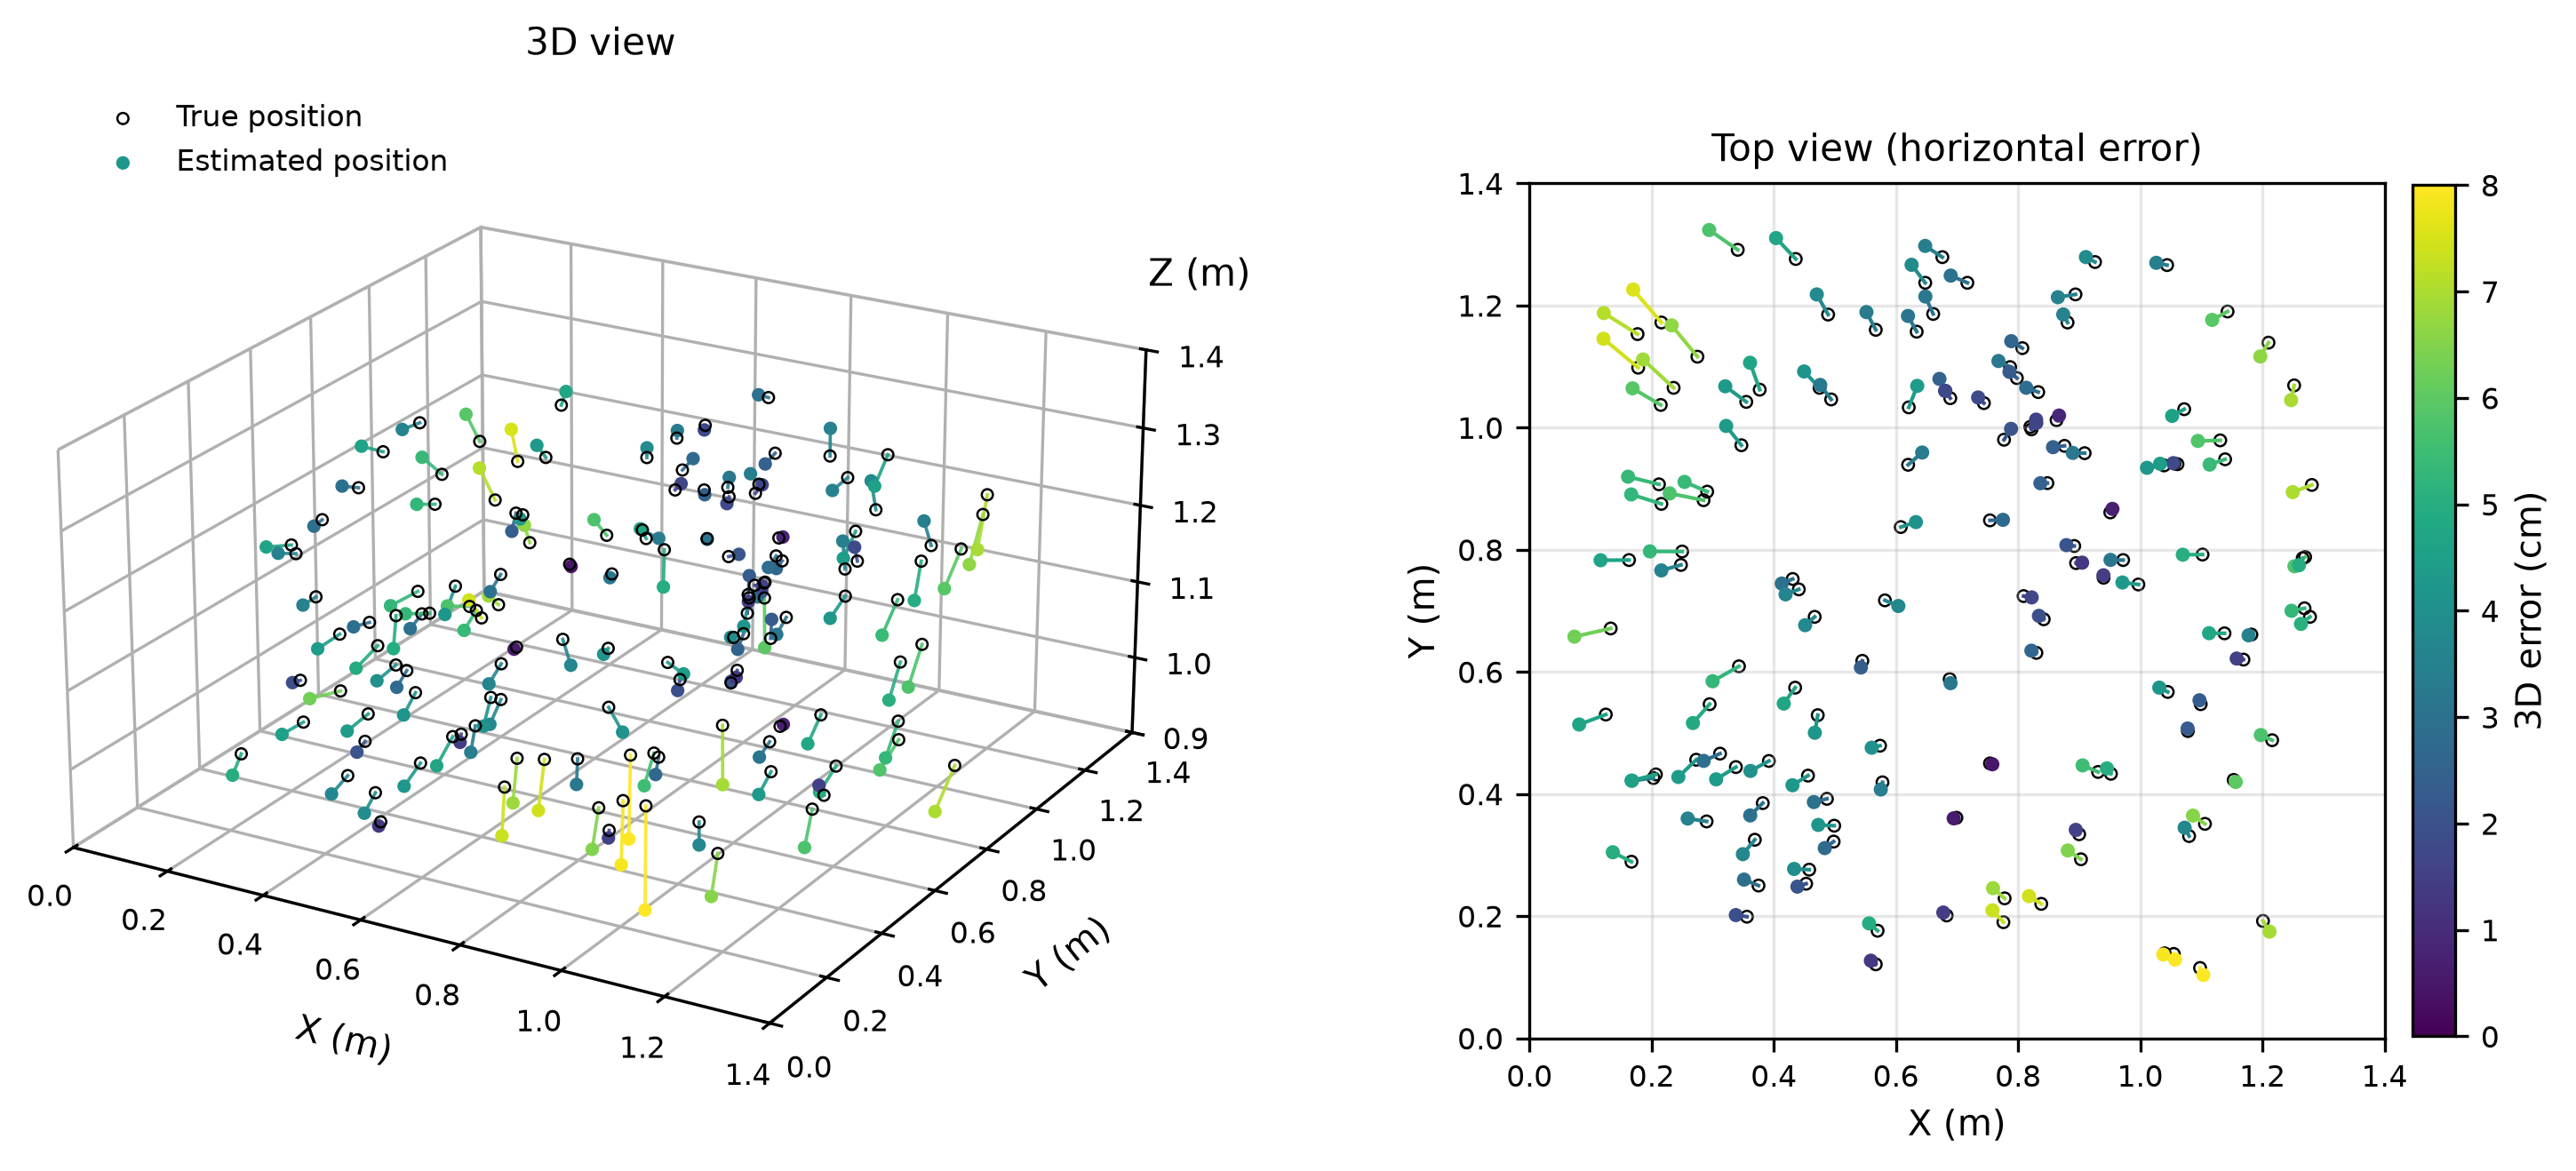
\includegraphics[width=\linewidth]{fig_demo_3d.png}
\caption{Live demo: 131 random positions, single LED, $K=5$. True positions (hollow) and estimates
(coloured by 3D error), joined by their error vectors.}\label{fig:demo}
\end{figure}

\section*{3. Key findings}
\begin{enumerate}[label=\textbf{F\arabic*.},leftmargin=8mm]
\item \textbf{Centimetre-level 3D positioning from one LED and one PD} (Fig.~\ref{fig:demo}).
  \begin{itemize}
  \item Direction and range come from the same $K$ RSS. No extra cooperative measurement is needed.
  \item $K=5$ performs like $K=10$, and $K=3$ still works without failures, but with no redundancy.
  \item The remaining error is dominated by model bias, not by noise: more orientations do not reduce
    it.
  \end{itemize}
\item \textbf{The PD angular response must be modelled correctly.} The shape test of the $K$ RSS
  selects the SQ model independently of $A$ and $m$. Lambertian receiver models fail by a factor of
  2 to 20.
\item \textbf{Self-calibration of the testbed geometry.} With the nominal $Z$ axis, the vertical bias
  grew linearly with height, and $A$, $m$ and the adapter tilt seemed to depend on the PD height.
  \begin{itemize}
  \item Two independent principles (amplitude and ray triangulation) both gave a $Z$ scale of
    0.63--0.65.
  \item A tape measurement then confirmed 0.6.
  \item With it, $A$ stays constant within $\pm0.2$\,\% and the adapter tilt within $\pm0.02^\circ$
    across heights.
  \end{itemize}
\item \textbf{Calibration budget: 9 well-placed points} (Fig.~\ref{fig:cal}). Only $A$ and $m$ are
  unknown.
  \begin{itemize}
  \item One point below the LED fixes $A$ but not $m$.
  \item Two points (nadir + one at $\approx20^\circ$) are the theoretical minimum, but fragile.
  \item A regular $3\times3$ or $4\times4$ grid over the working area reaches the full-map result
    (3.5--3.6\cm). Ten random points give 3.8\cm; points clustered near the LED fail.
  \item The reason: the measured pattern is \emph{not} a single $\cos^m$. The apparent $m$ drops from
    $\approx11$ near the axis to $\approx6$ beyond $20^\circ$. The calibration points must therefore
    cover the angles used for positioning. The $\cos^m$ model floor is 3.1\cm.
  \item The same 9 points also calibrate the LED $XY$ (within 3\,mm, 3.5\cm\ error). The LED
    \emph{height} cannot be identified from a single plane: it must be measured, or a second plane is
    needed.
  \end{itemize}
\item \textbf{Installation diagnosis of the other LEDs} (Fig.~\ref{fig:leds}). The 9-point
  calibration gives the same result as the full map for every LED, but the 300, 900 and 700\,kHz LEDs
  position worse (6--17\cm) because they are not pointing straight down.
  \begin{itemize}
  \item Their pattern centres are shifted by 2.6, 6 and 18\cm\ from their physical positions, i.e.\
    tilts of $\approx0.8^\circ$, $1.9^\circ$ and $5.4^\circ$.
  \item The calibration of a flat-PD plane alone cannot separate an LED tilt from an LED offset.
  \end{itemize}
\item \textbf{Multi-LED, directions only.} Intersecting the directions to several LEDs needs neither
  the LED power nor $A$ and $m$.
  \begin{itemize}
  \item \textbf{Two LEDs} are enough, the realistic case of a corridor, and the minimum to cross rays
    and to estimate the yaw. With the best pair (500 + 900\,kHz): 3.3\cm\ with known yaw, 3.6\cm\
    estimating the yaw too (1.2$^\circ$ yaw error).
  \item With the four LEDs: 2.8\cm\ and 2.9\cm\ (0.7$^\circ$ yaw error).
  \item The pairs that include the tilted 700\,kHz LED are the worst (6.3\cm), consistent with F5.
  \end{itemize}
\item \textbf{Acquisition time is dominated by the rotation stage.}
  \begin{itemize}
  \item 3.7\,min per position with $K=5$ (live demo average) and 4.2\,min with $K=10$.
  \item About 86\,\% of that time is the MTRS rotation at 1.5$^\circ$/s; the measurements themselves
    take a few seconds.
  \item By estimate, a rotation stage of $\sim20^\circ$/s would bring a $K=5$ position below one
    minute: faster demos, larger datasets and moving receivers.
  \end{itemize}
\end{enumerate}

\begin{figure}[H]\centering
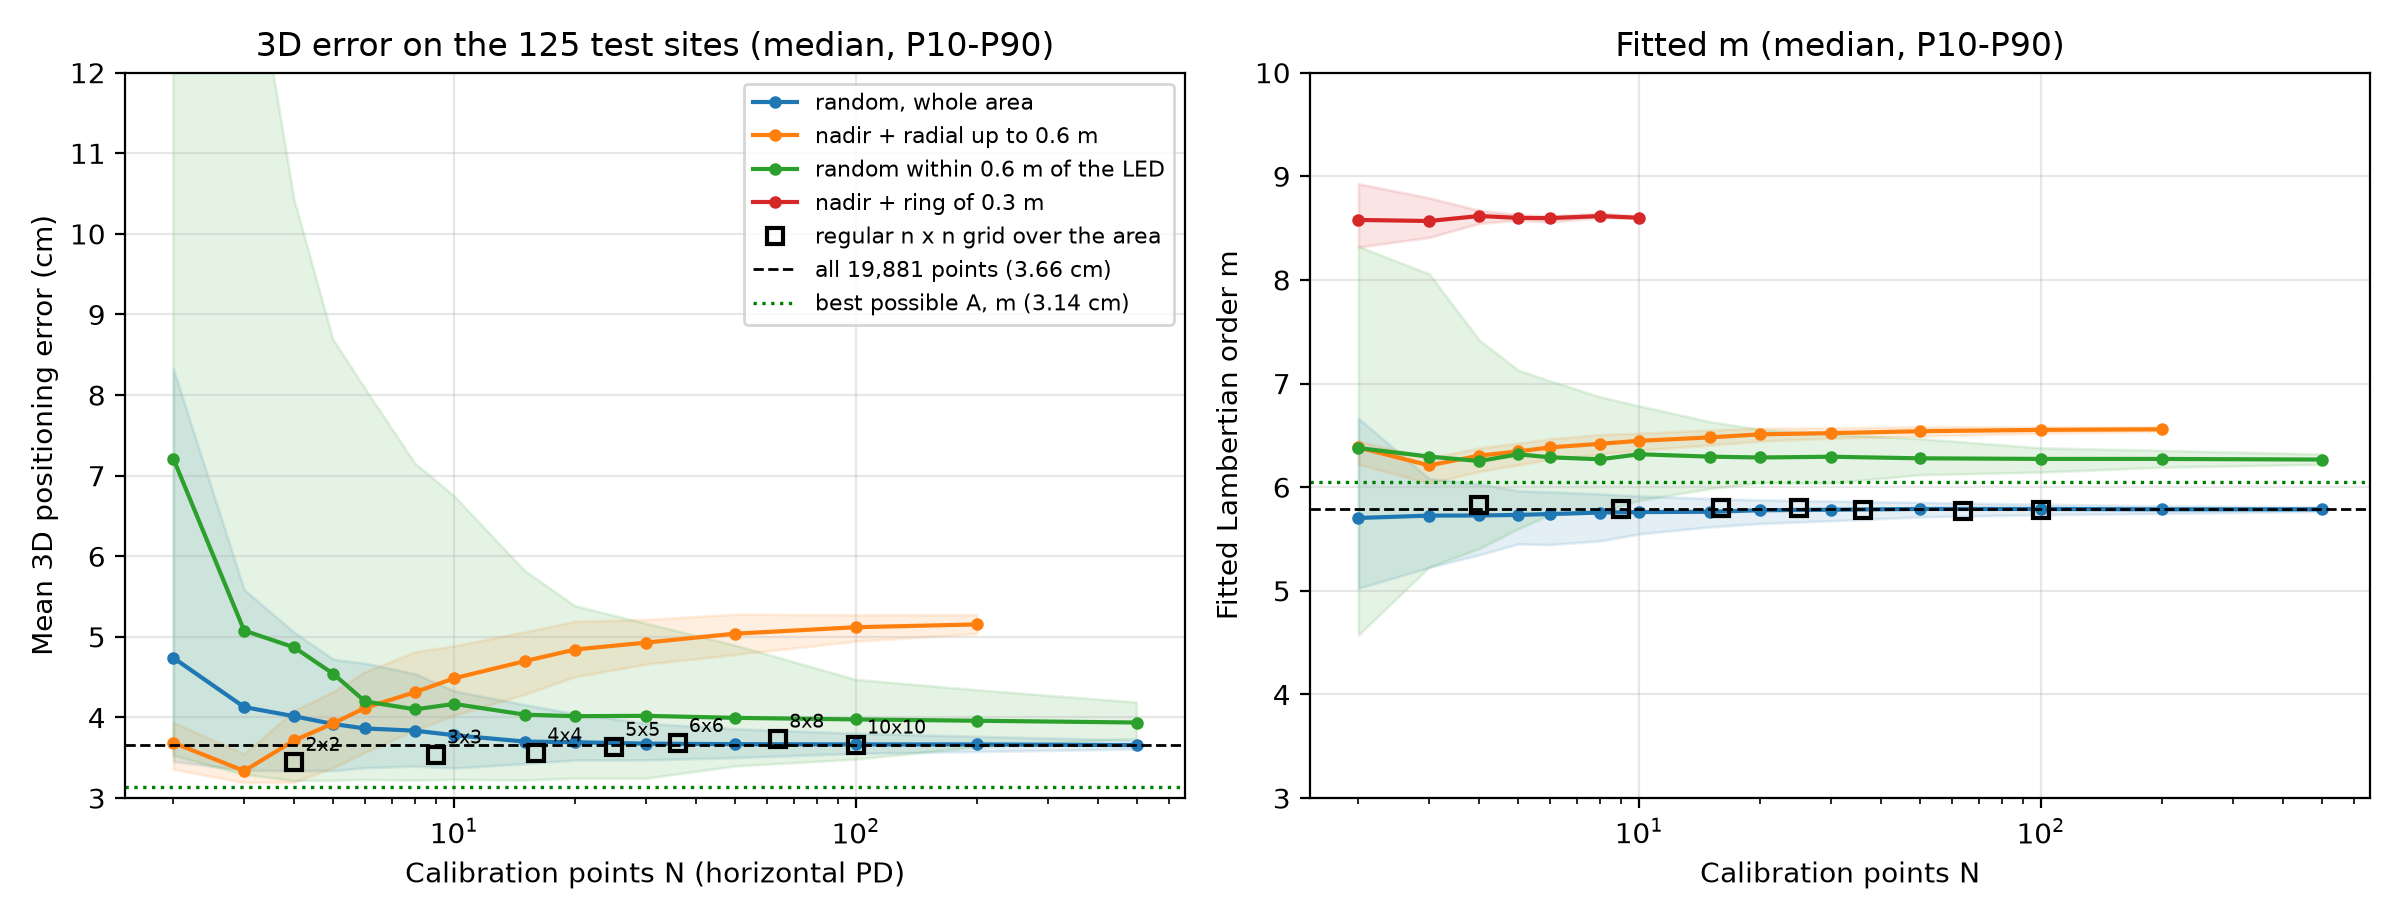
\includegraphics[width=0.92\linewidth]{../Calibration/figures/error_vs_N.png}
\caption{Calibration budget (500\,kHz LED, flat PD): 3D error on the 125 positions vs.\ number of
calibration points for several layouts (left) and the fitted $m$ (right). Squares: regular $n\times n$
grids over the working area.}\label{fig:cal}
\end{figure}

\begin{figure}[H]\centering
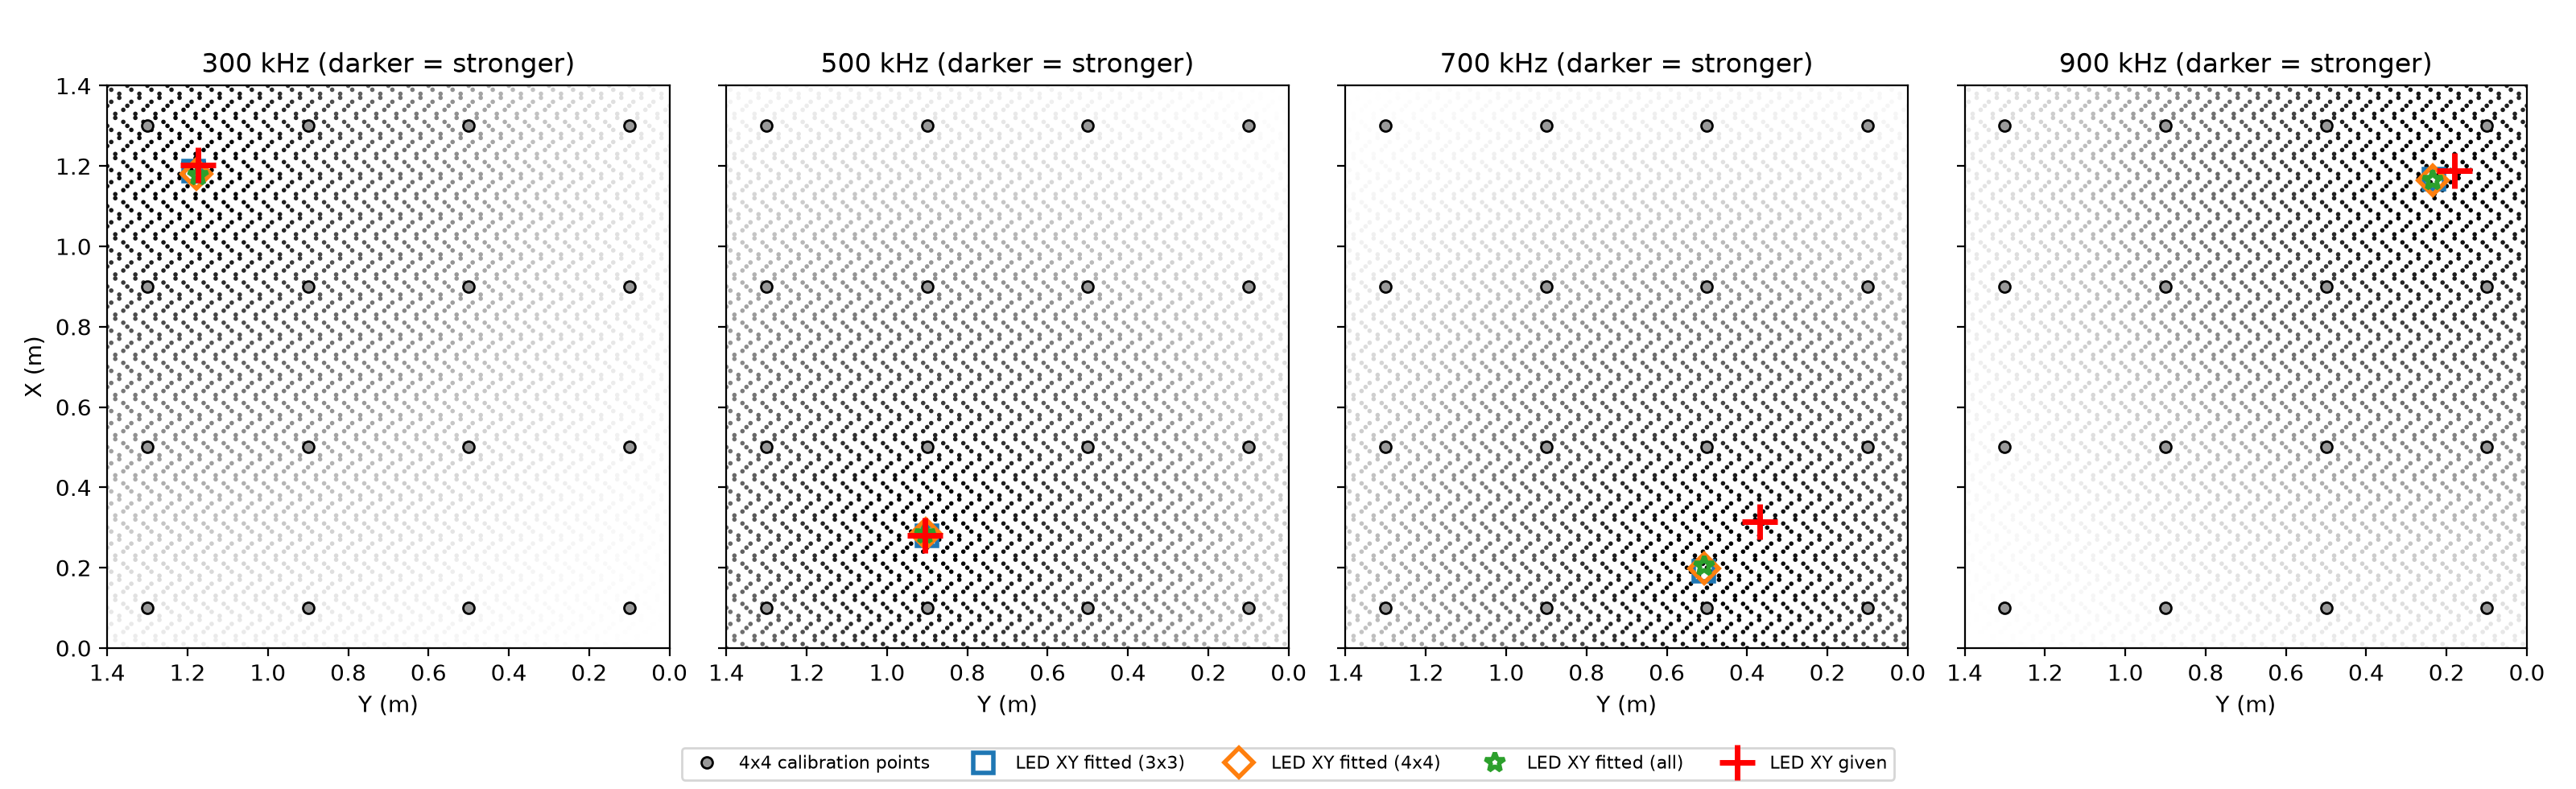
\includegraphics[width=0.95\linewidth]{../Calibration/figures/other_leds_maps.png}
\caption{Flat-PD RSS map of each LED. Markers: the LED $XY$ fitted from the calibration points (centre
of the radiation pattern) and the physical LED position (red cross). The 700\,kHz LED shows an 18\cm\
offset, i.e.\ a $\approx5^\circ$ tilt.}\label{fig:leds}
\end{figure}

\section*{4. Most promising directions}
\begin{enumerate}[leftmargin=6mm]
\item \textbf{Journal paper on the experimental validation} (immediate).
  \begin{itemize}
  \item A dense regular 3D grid plus a blind random test set, with a strict calibration/test split.
  \item Comparison with the position error bound (PEB), using the noise measured from repeated
    records.
  \item The calibration budget and the self-diagnosis results as methodological contributions.
  \end{itemize}
\item \textbf{A better LED pattern model} to break the 3.1\cm\ floor of $\cos^m$: an angle-dependent
  $m$, a spline, or a physics-informed NN. Calibrating on \emph{two} planes would also identify the LED
  height and tilt.
\item \textbf{Two-LED / multi-LED positioning with yaw estimation}: towards IMU-free 3D position
  \emph{and} attitude for mobile receivers (corridors, drones). Next step: fusing directions and
  ranges.
\item \textbf{Robustness studies.}
  \begin{itemize}
  \item Arbitrary but known orientations (no fixed codebook).
  \item Orientation errors (an IMU instead of encoders).
  \item Occlusion of some orientations: detect them (e.g.\ with the residual of the RSS-shape fit) and
    estimate with the remaining ones. The results above with $K=5$ and $K=3$ suggest that a reduced
    set of orientations can still position.
  \end{itemize}
\item \textbf{Faster acquisition.} A faster rotation stage (F7), continuous rotation with on-the-fly
  sampling (hundreds of orientations in the time of $K=10$), or a pyramid angle-diversity receiver for
  snapshot positioning.
\item \textbf{Data for machine learning.} A dense, angle-major dataset (one MTRS angle per scan) could
  provide $\sim$30\,000 labelled measurements in one day, for a hybrid model-based/learning
  collaboration.
\end{enumerate}

\section*{5. Equipment requests}
\begin{itemize}
\item \textbf{Faster motorized rotation stage} ($\gtrsim 20^\circ$/s): the current stage is the
  bottleneck of every experiment (F7).
\item \textbf{Automatic laser distance meter}: to measure the PD and LED heights and positions quickly
  and reproducibly. Today the ground truth of the heights relies on a tape (F3, F4).
\item \textbf{IMU} on the receiver: orientation measured with realistic errors, needed for the
  robustness study and the step towards drones.
\end{itemize}

\section*{6. Points to discuss}
\begin{enumerate}[leftmargin=6mm]
\item \textbf{Journal timing.} Are the current results, together with the theory (receiver-side
  reorientation, PEB), enough to start writing the journal paper? Or should the writing wait for the
  dense 3D grid, the blind test set and the PEB comparison?
\item \textbf{Scope and venue.} Single LED only, or also include the two-LED / multi-LED results?
  Target journal (e.g.\ IEEE TIM, IEEE Sensors Journal or IEEE IoT Journal)?
\item \textbf{Equipment.} Priority and budget of the rotation stage, the laser distance meter and the
  IMU.
\item \textbf{LED installation.} Realign the tilted LEDs (700\,kHz), or keep them and model the LED tilt
  (a more general calibration, but not comparable with the data already recorded)?
\item \textbf{Collaborations.} Scope of a possible collaboration on machine learning and of data
  sharing.
\end{enumerate}

\end{document}
